\documentclass{article}
\usepackage{hyperref}
\usepackage{graphicx}

\title{OO: Analiza zbirke, poročilo}
\date{\today}
\author{Jan Anžur, Matija Jemec in Niko Šneberger}

\begin{document}

	\maketitle
	\pagenumbering{gobble}
	\newpage
	\pagenumbering{arabic}

	\section{Opis}

		Namen projekta je analiza in primerjava umetniških slik iz različnih obdobij.
		Iz slik smo zbrali več vrst podatkov:

		\begin{itemize}
			\item lokacije in število \textbf{obrazov} na sliki,
			\item lokacije in število \textbf{teles},
			\item lokacije in število \textbf{črt},
			\item lokacije in število \textbf{kontur} in
			\item \textbf{histogram}.
		\end{itemize}

		Nato smo slike razvrstili po časovnih obdobjih in nato naredili podobno analizo
		po obdobjih.

		Navodila za uporabo se nahajajo v datoteki \texttt{readme.md}.

	\newpage

	\section{Histgrami obdobij}
		Za vsako obdobje smo zgenerirali histogram barv.
		Ostali statistični podatki so na voljo preko spletne strani.

		\begin{center}
			\begin{tabular}{cc}

				\noindent
				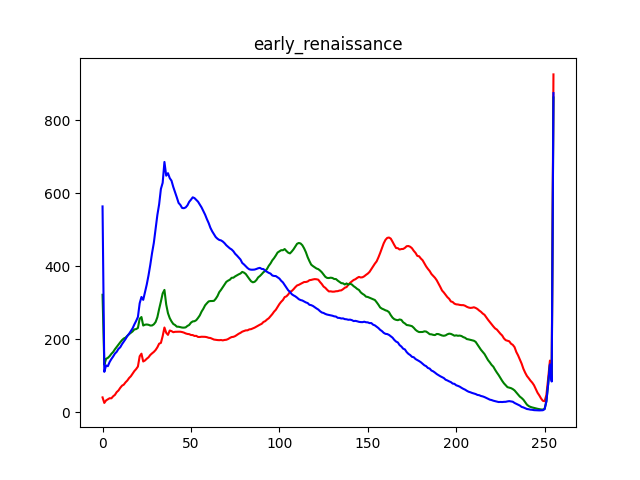
\includegraphics[width=0.5\textwidth]{plots/early_renaissance.png}
				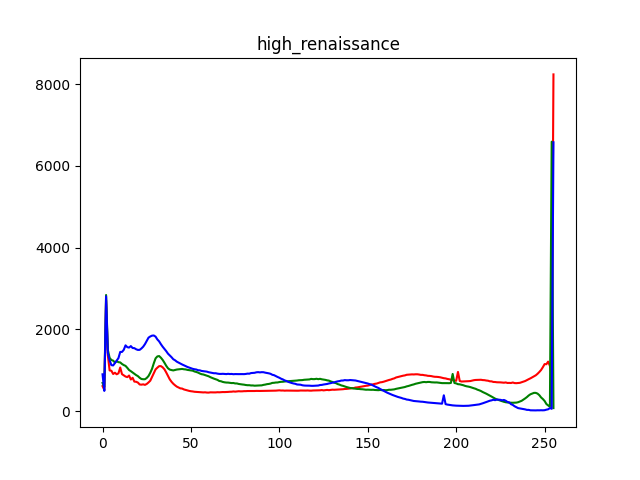
\includegraphics[width=0.5\textwidth]{plots/high_renaissance.png}\\[2em]
				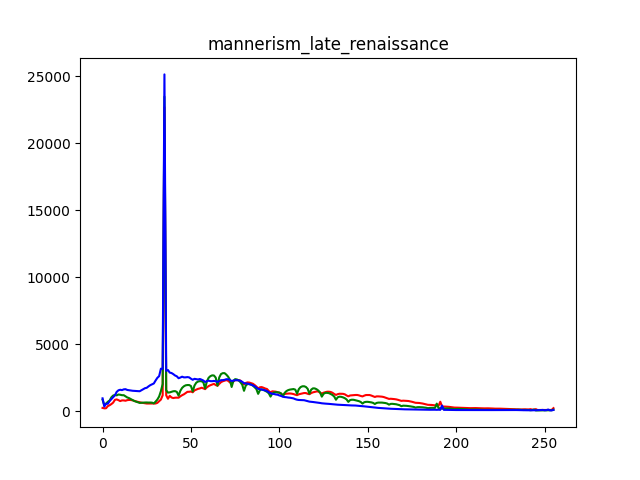
\includegraphics[width=0.5\textwidth]{plots/mannerism_late_renaissance.png}
				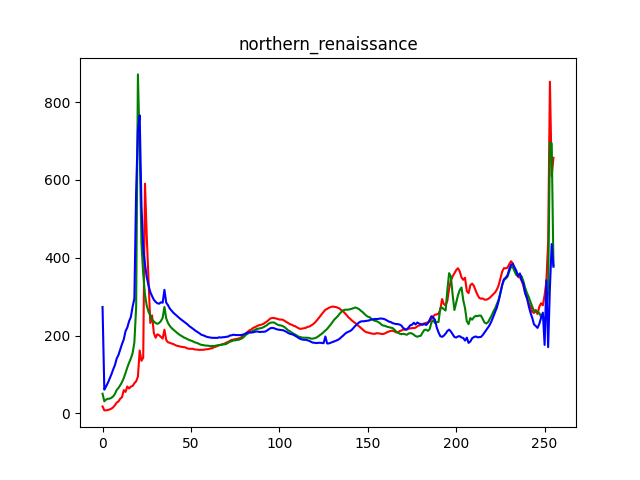
\includegraphics[width=0.5\textwidth]{plots/northern_renaissance.png}\\[2em]
				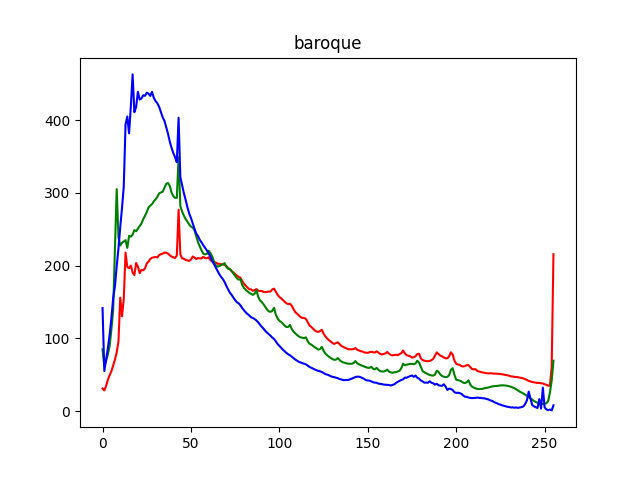
\includegraphics[width=0.5\textwidth]{plots/baroque.png}
				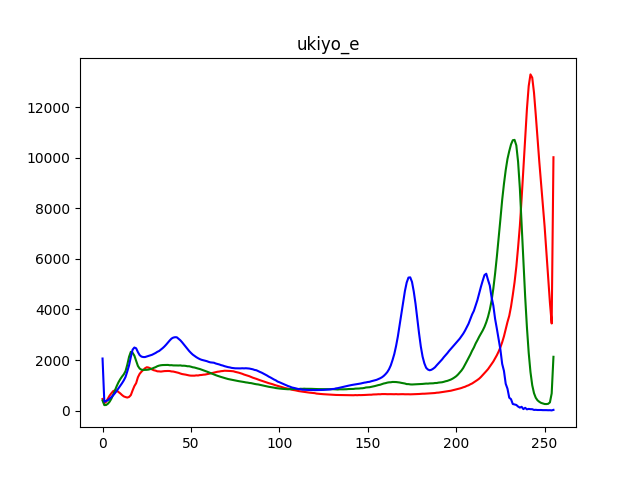
\includegraphics[width=0.5\textwidth]{plots/ukiyo_e.png}\par

			\end{tabular}
		\end{center}
		\newpage

		\begin{center}
			\begin{tabular}{cc}

				\noindent
				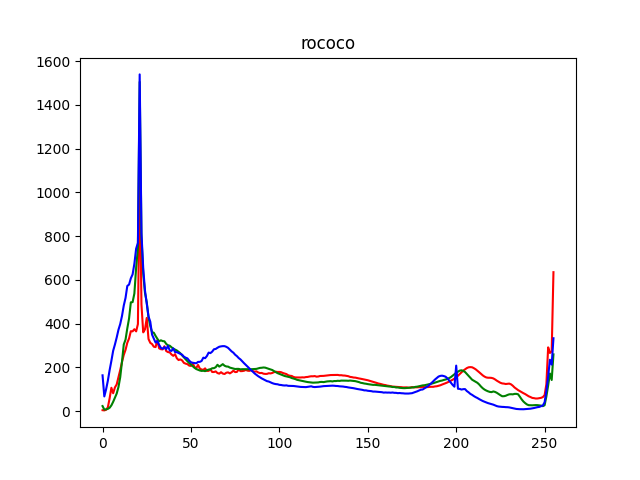
\includegraphics[width=0.5\textwidth]{plots/rococo.png}
				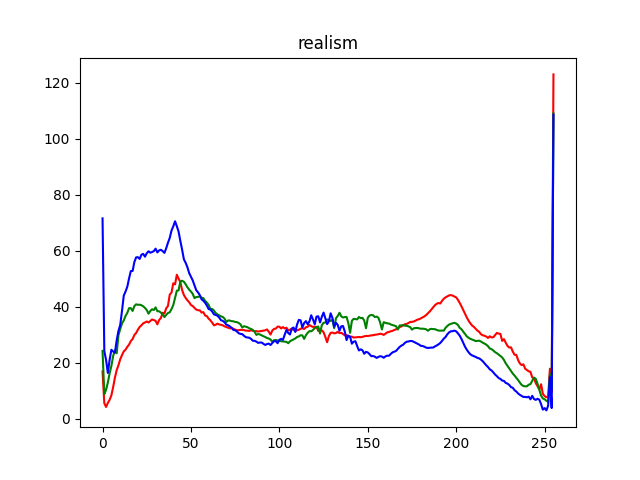
\includegraphics[width=0.5\textwidth]{plots/realism.png}\\[2em]
				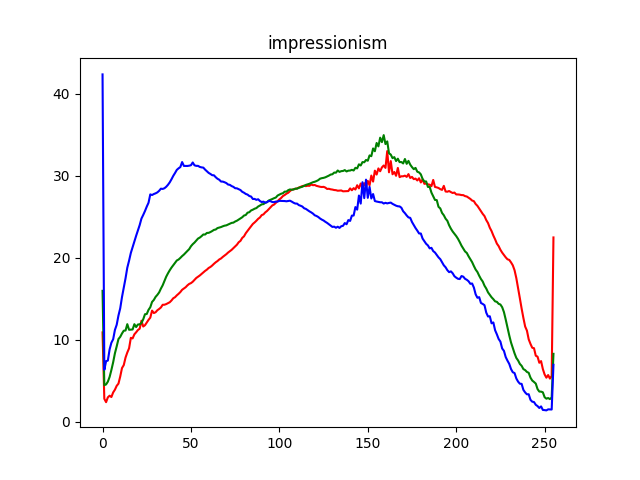
\includegraphics[width=0.5\textwidth]{plots/impressionism.png}
				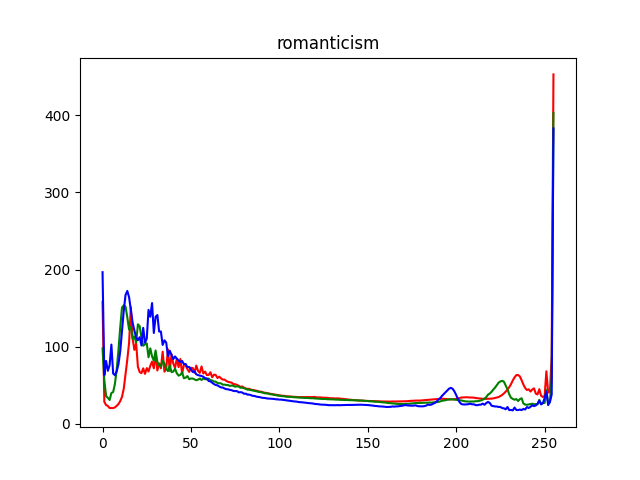
\includegraphics[width=0.5\textwidth]{plots/romanticism.png}\\[2em]
				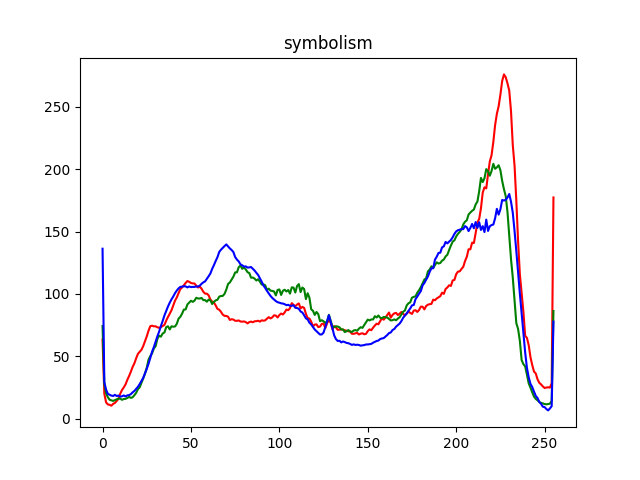
\includegraphics[width=0.5\textwidth]{plots/symbolism.png}
				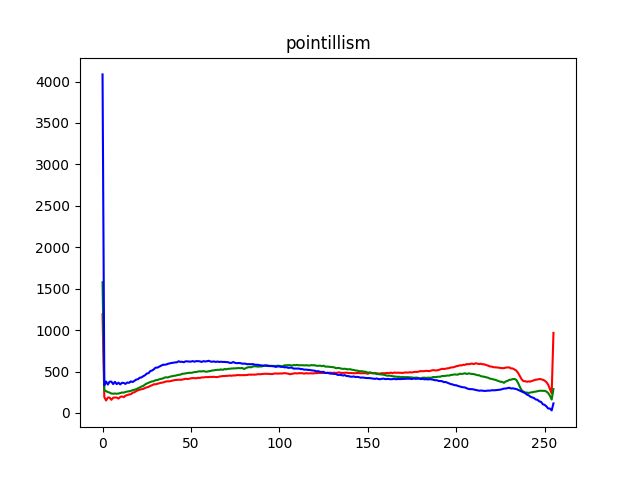
\includegraphics[width=0.5\textwidth]{plots/pointillism.png}\par

			\end{tabular}
		\end{center}
		\newpage

		\begin{center}
			\begin{tabular}{cc}

				\noindent
				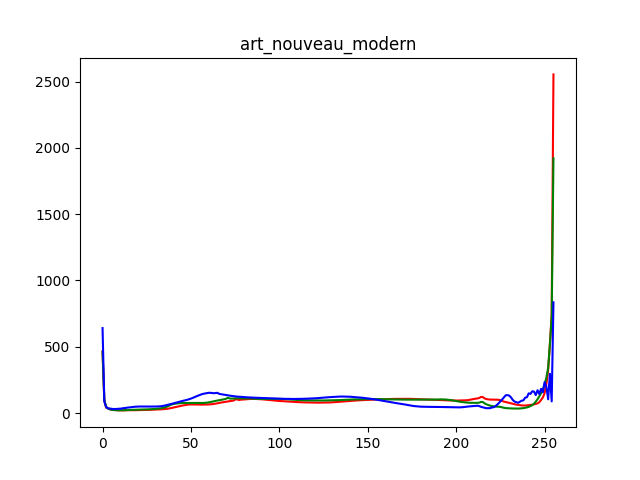
\includegraphics[width=0.5\textwidth]{plots/art_nouveau_modern.png}
				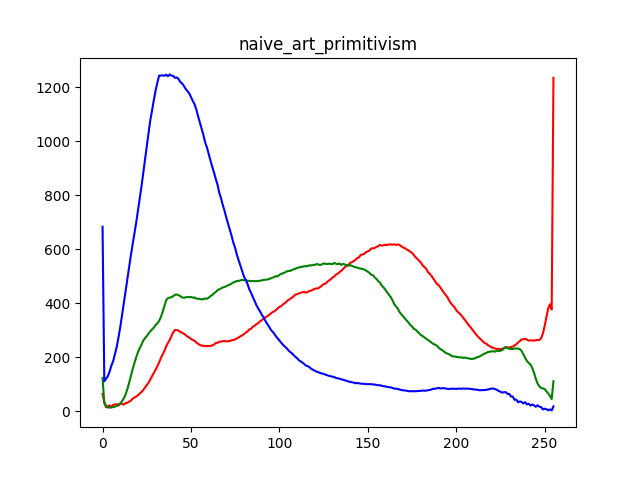
\includegraphics[width=0.5\textwidth]{plots/naive_art_primitivism.png}\\[2em]
				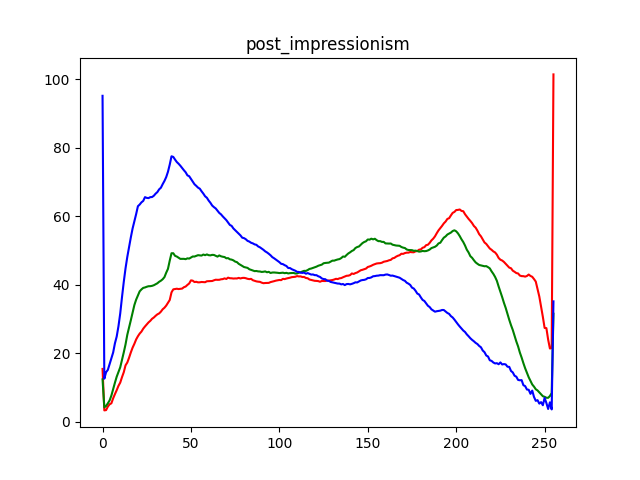
\includegraphics[width=0.5\textwidth]{plots/post_impressionism.png}
				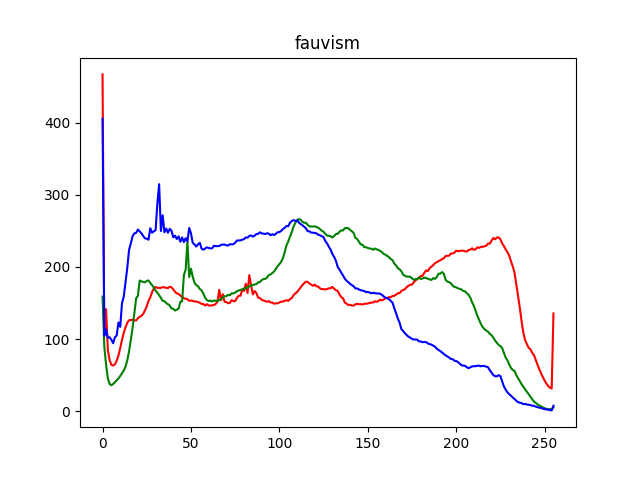
\includegraphics[width=0.5\textwidth]{plots/fauvism.png}\\[2em]
				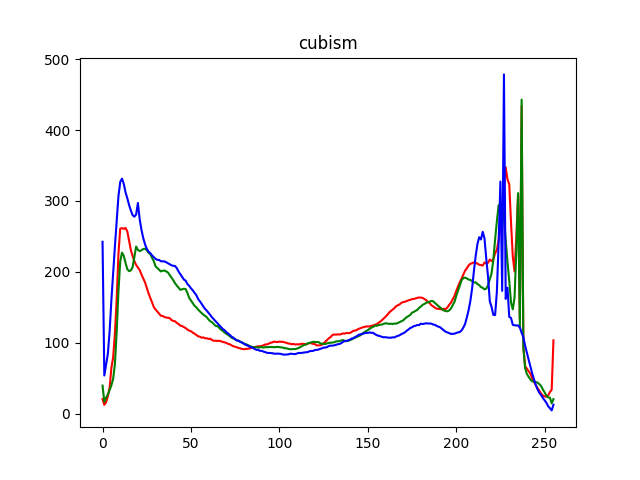
\includegraphics[width=0.5\textwidth]{plots/cubism.png}
				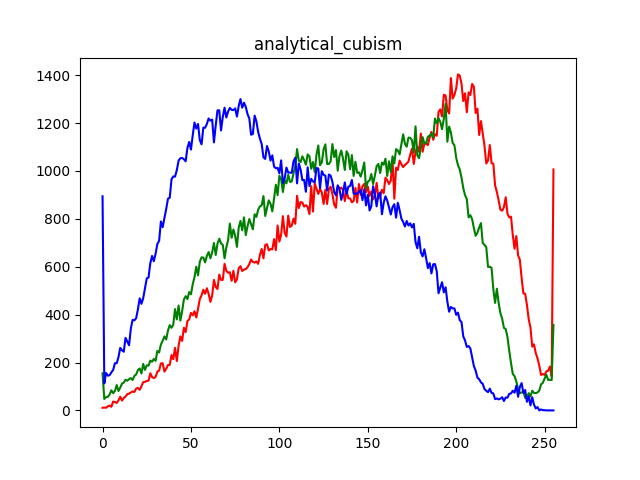
\includegraphics[width=0.5\textwidth]{plots/analytical_cubism.png}\par

			\end{tabular}
		\end{center}
		\newpage

		\begin{center}
			\begin{tabular}{cc}

				\noindent
				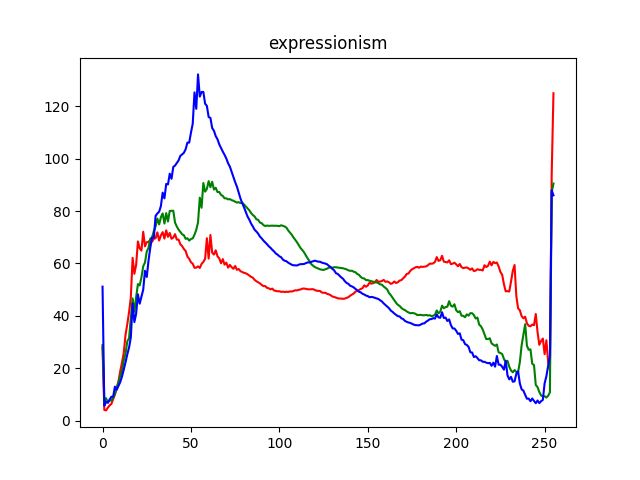
\includegraphics[width=0.5\textwidth]{plots/expressionism.png}
				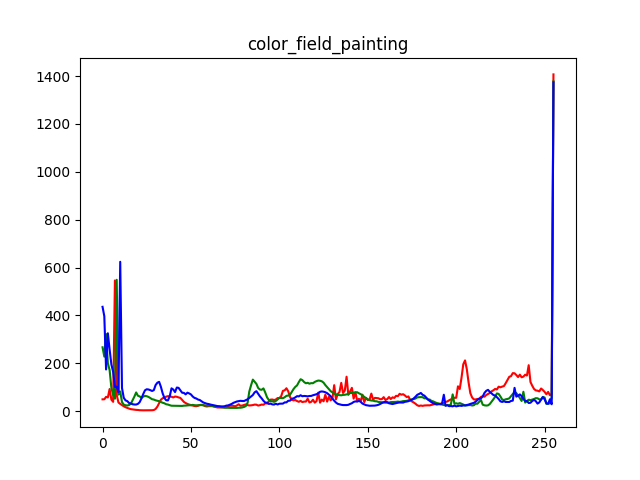
\includegraphics[width=0.5\textwidth]{plots/color_field_painting.png}\\[2em]
				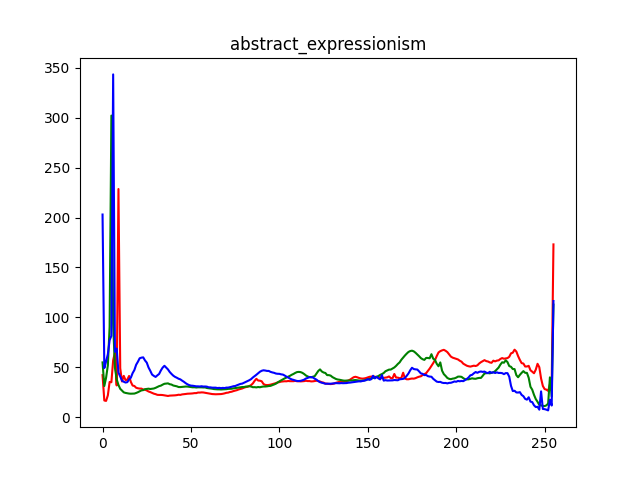
\includegraphics[width=0.5\textwidth]{plots/abstract_expressionism.png}
				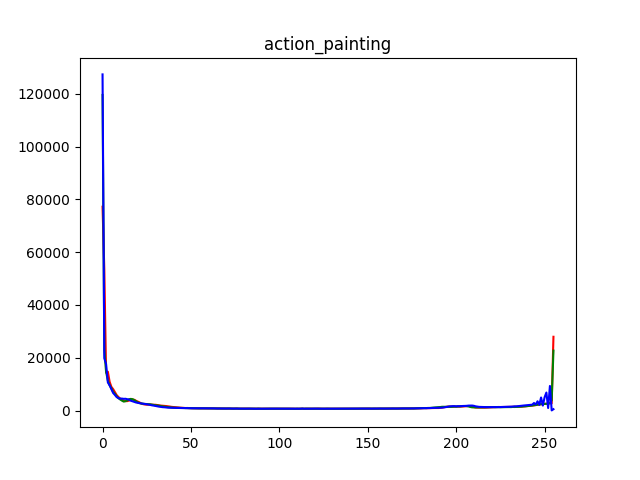
\includegraphics[width=0.5\textwidth]{plots/action_painting.png}\\[2em]
				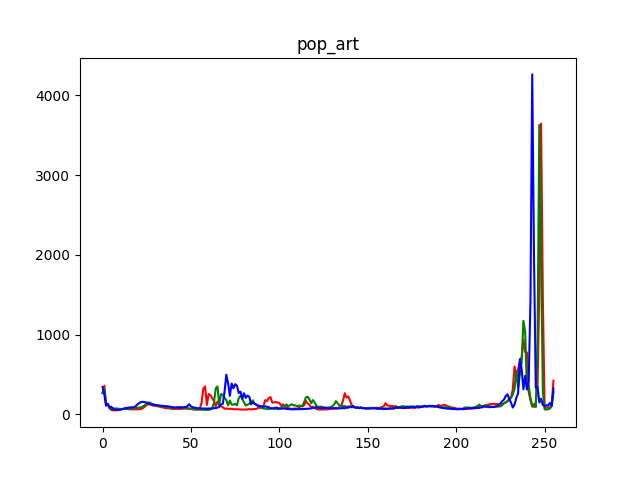
\includegraphics[width=0.5\textwidth]{plots/pop_art.png}
				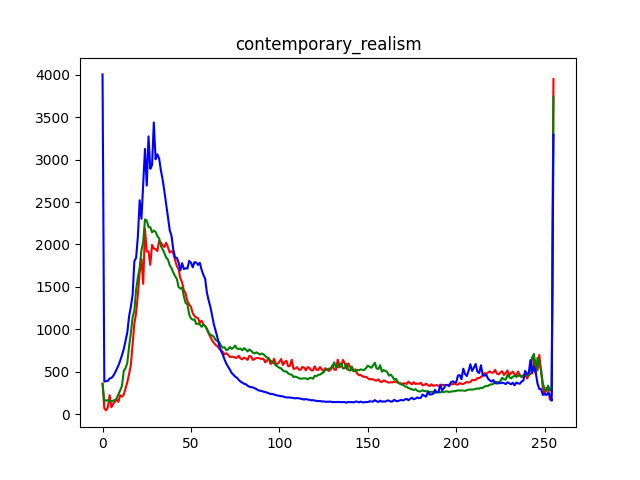
\includegraphics[width=0.5\textwidth]{plots/contemporary_realism.png}\par

			\end{tabular}
		\end{center}
		\newpage

		\begin{center}
			\begin{tabular}{cc}

				\noindent
				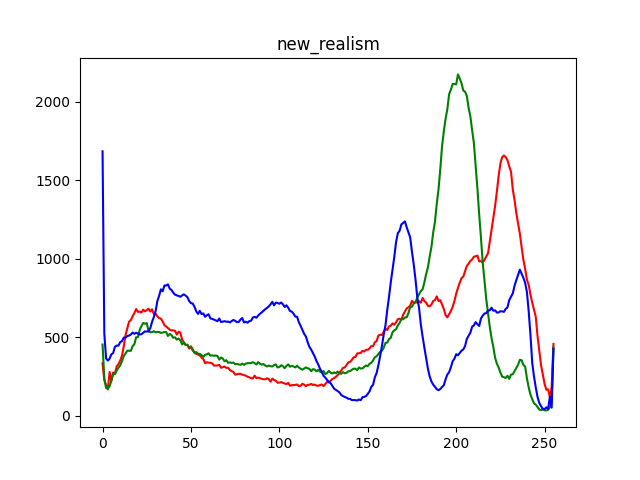
\includegraphics[width=0.5\textwidth]{plots/new_realism.png}
				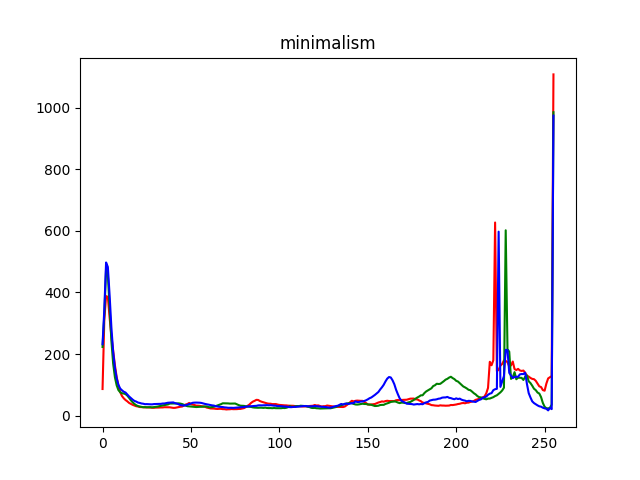
\includegraphics[width=0.5\textwidth]{plots/minimalism.png}\par

			\end{tabular}
		\end{center}
		\newpage


	\section{Reference}
		Pri projektu smo analizirali slike iz zbirke \href{https://www.wikiart.org/}{WikiArt}.

	\section{Porazdelitev dela}
		\begin{itemize}
			\item Jan A.: odjemalec in strežnik za spletno stran, generiranje JSON označb
			\item Matija J.: detekcija teles, črt in kontur, histogrami, komunikacija z API za WikiArt
			\item Niko Š.: detekcija obrazov, generiranje kolekcij slik za obdobja in izdelava predstavitvenega videa
		\end{itemize}

\end{document}
